\section{Results}
\numberwithin{equation}{section}

\subsection{Setup of the testing environment}

The benchmarks were conducted on a GPU cluster consisting of 12 compute nodes,
each equipped with a quad core Intel Xeon CPU E5-2609 CPU (2.40GHz), 64GB RAM
and 4 NVIDIA Tesla K20M GPUs. Job submission to the compute nodes can be done
using QSUB \cite{qsub}. The used gain medium is a \textbf{TODO: Daniel should
check/complete the description of the medium} YAG crystal with a square surface
of $16cm^2$\textbf{(?)} and a thickness of $0.6cm$\textbf{(?)}. Its upper
surface was sampled with 321 points, resulting in 600 Delaunay triangles (see
section \ref{subsec:meshSampling}). The mesh is extruded 9 times on the vertical
axis, amounting to a total of 3210 sample points and 5400 prisms respectively.



\subsection{Benchmark of values}

\begin{itemize}

  \item TODO

  \item \textbf{Image: gain VS time for one single point. Overlay between
    experiment/daniels sim/our sim}

  \item comparison with previous values from Daniel's thesis

  \item (comparison with results from an experiment)

\end{itemize}



\subsection{Runtimes}
In Figure \ref{plot:runtime}, the runtimes of the original single threaded
algorithm from \cite{ASE2010} are compared to the developed non-adaptive
parallel ASE-flux algorithm with different numbers of rays to demonstrate
scaling for different workloads. All simulations were done without the usage
of reflections. To increase the number of GPUs to 48, a QSUB
array job was scheduled and the sampling points distributed to the available
GPUs as seen in section \ref{subsubsec:multigpu}.  When using the CPU or up to 4
GPUs, the computation uses only a single node, which results in a linear scaling
of the algorithm. If the cluster's job submission system is used, a significant
runtime overhead can be seen as a result of the job scheduler. Therefore, using
a high number of GPUs can lead to suboptimal performance in otherwise fast
computations. However, this becomes neglegible for very work intensive
simulations.
\begin{figure}[H]
  \centerline{
    \resizebox{0.5\textwidth}{!}{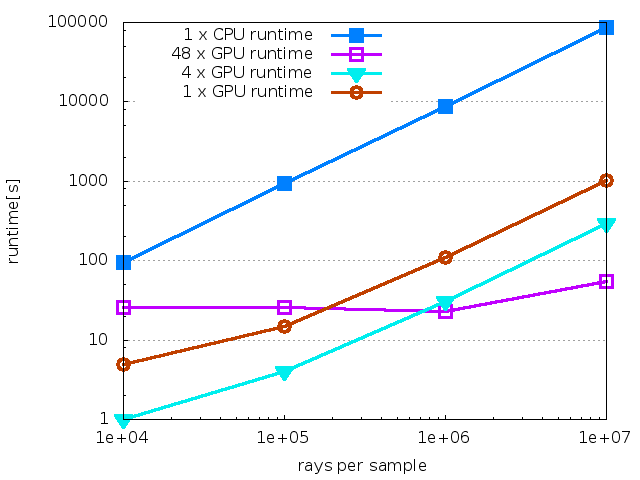
\includegraphics{plot/runtime.png}}}
  \caption{runtime of orginial algorithm compared to parallel algorithm}
  \label{plot:runtime}
\end{figure}
Apart from scheduling overhead, distributing the computation to multiple devices
scales well as long as every sample point is simulated with the exact same
number of rays. Changing this (e.g. through adaptive sampling), leads to a
potentially unbalanced workload on different devices and a high impact on efficiency.
(Figure \ref{plot:gpu_scaling}).
\begin{figure}[H]
  \centerline{
    \resizebox{0.5\textwidth}{!}{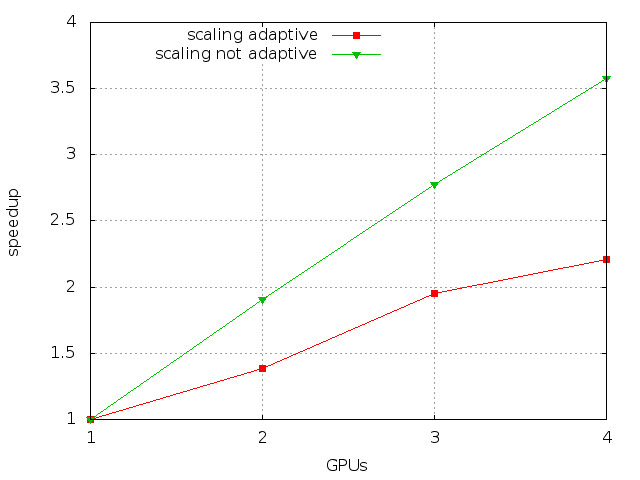
\includegraphics{plot/scaling.png}}}
  \caption{efficiency on multiple devices}
  \label{plot:gpu_scaling}
\end{figure}
Nevertheless, by using the idea of adaptive sampling, the precision of the
simulation can be adjusted using a $MSE$-threshold rather than simply increasing
the number of rays for all the sample points. Since only a small number of
sample points actually needs to be sampled with a high resolution, a small
increase in runtime can be sufficient to lower the maximal $MSE$ values below
the desired threshold. (Figure
\ref{plot:adaptive_runtime}). This can be adjusted to yield similar simulation
results as the non-adaptive implementation at a fraction of the runtime. Note
that some values in the graphic actually display almost the same runtime, since
the computation always succeeded to stay below the given threshold with very
little additional effort.
\begin{figure}[H]
  \centerline{
    \resizebox{0.5\textwidth}{!}{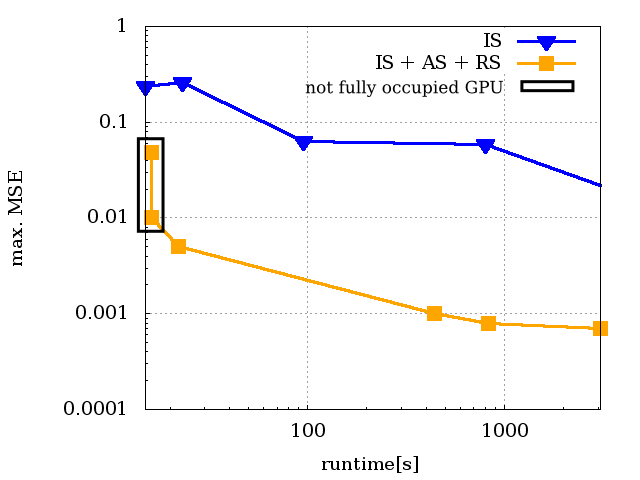
\includegraphics{graphics/adaptive_runtime.png}}}
  \caption{runtime comparison of adaptive and non adaptive }
  \label{plot:adaptive_runtime}
\end{figure}
\subsection{Limitations and future work}
\label{subsec:limitations}
Future work should address reflections on the lateral sides of the gain medium
to allow the simulation of lateral feedback. The current implementation only
supports reflections on the upper and lower surface. Apart from that, the
scaling issues seen in Figure \ref{plot:gpu_scaling} can be mitigated by
assigning the sample points to the GPUs in a demand-based way. In theory,
processing times on the different devices will be more evenly, reducing the time
needed to wait for the slowest device and thus decreasing the overall duration
of the calculation. This might be efficiently by allocating the nodes first and
then using Message Passing Interface (MPI)\cite{MPI} to assign sample points by
a on-demand basis to the nodes. Lastly, a faster job submission system than QSUB
could improve the previously mentioned scheduling overhead significantly.
